\documentclass[12pt,a4paper]{article}

% Line numbers

% Font setup

  \usepackage[default,tabular,lf]{sourcesanspro}
  \usepackage[cmintegrals]{newtxsf}
  \usepackage[italic,eulergreek]{mathastext}

% Encoding & language
\usepackage[T1]{fontenc}
\usepackage[utf8]{inputenc}
%\usepackage[australian]{babel}

% Geometry & spacing
\usepackage{geometry}
\geometry{left=2cm,right=2cm,top=2.5cm,bottom=2.5cm}
\usepackage{microtype}
\usepackage{setspace}
\setstretch{1.2}
\setlength{\parskip}{6pt plus 2pt minus 1pt}
\setlength{\parindent}{0pt}
\setlength{\emergencystretch}{3em}

% Graphics & tables
\usepackage{graphicx,float,booktabs,longtable}
\usepackage{multirow}
\usepackage{array}
%\usepackage{tabu}
\setcounter{topnumber}{2}
\setcounter{bottomnumber}{2}
\setcounter{totalnumber}{4}
\renewcommand{\topfraction}{0.85}
\renewcommand{\bottomfraction}{0.85}
\renewcommand{\textfraction}{0.15}
\renewcommand{\floatpagefraction}{0.8}

\usepackage{longtable,booktabs}
% Fix footnotes in tables (if needed)
\IfFileExists{footnote.sty}{
  \usepackage{footnote}
  \makesavenoteenv{longtable}
}{}

% Automatically reduce font size in tables
%\usepackage{etoolbox}
%\AtBeginEnvironment{longtable}{\footnotesize}
%\AtBeginEnvironment{tabular}{\footnotesize}

% Hyperlinks
\usepackage{xcolor}
\definecolor{darkblue}{rgb}{0,0,.6}
\usepackage{hyperref}
\hypersetup{
  colorlinks=true,
  linkcolor=darkblue,
  citecolor=darkblue,
  urlcolor=darkblue,
  breaklinks=true,
  bookmarksopen=true,
  bookmarksnumbered=true
}
\urlstyle{same}

% Header/Footer
\usepackage{fancyhdr}
\pagestyle{fancy}
\fancyhf{}
\lhead{\textsf{\nouppercase{\leftmark}}}
\rhead{\textsf{\thepage}}
\setlength{\headheight}{15pt}
\renewcommand{\headrulewidth}{0.4pt}

% Captions
\usepackage{caption}
\DeclareCaptionStyle{italic}[justification=centering]{labelfont={bf},textfont={it},labelsep=colon}
\captionsetup[figure]{style=italic,format=hang,singlelinecheck=true}
\captionsetup[table]{style=italic,format=hang,singlelinecheck=true}

% Bibliography
\usepackage[style=authoryear-comp,backend=biber,natbib=true]{biblatex}
\ExecuteBibliographyOptions{bibencoding=utf8,minnames=1,maxnames=3,maxbibnames=99,dashed=false,terseinits=true,giveninits=true,uniquename=false,uniquelist=false,doi=false,isbn=false,url=true,sortcites=false}
\DeclareFieldFormat{url}{\texttt{\url{#1}}}
\DeclareFieldFormat[article]{volume}{\mkbibbold{#1}}
\DeclareFieldFormat[article]{number}{\mkbibparens{#1}}
\DeclareFieldFormat[article]{title}{\MakeCapital{#1}}
\DeclareFieldFormat[inproceedings]{pages}{\lowercase{pp.~}#1}
\renewbibmacro{in:}{\ifentrytype{article}{}{\printtext{\bibstring{in}\intitlepunct}}}
\AtEveryBibitem{\clearfield{month}}
\AtEveryCitekey{\clearfield{month}}
\addbibresource{abundance-decline.bib}
\addbibresource{packages.bib}

% Section titles
\usepackage[compact,sf,bf]{titlesec}
\titleformat{\section}[block]{\fontsize{15}{17}\bfseries\sffamily}{\thesection}{0.4em}{}
\titleformat{\subsection}[block]{\fontsize{12}{14}\bfseries\sffamily}{\thesubsection}{0.4em}{}
\titlespacing{\section}{0pt}{*3}{*1}
\titlespacing{\subsection}{0pt}{*1}{*0.5}

% Title block with optional branding
\usepackage{titling}
\usepackage[absolute,overlay]{textpos}
\setlength{\TPHorizModule}{1cm}
\setlength{\TPVertModule}{1cm}

% Abstract box styling
\usepackage{tcolorbox}
\newenvironment{abstractbox}
  {\begin{tcolorbox}[colback=gray!5!white,colframe=gray!50!black,
  width=\textwidth, boxrule=1.0pt, sharp corners, left=4pt, right=4pt, top=4pt, bottom=4pt]}
  {\end{tcolorbox}}

% Title metadata
\title{Three Decades of ESA-Listing: Are Snake River Spring/summer Chinook Salmon and Steelhead on the Path to Recovery?}

\author{%
\textbf{Ryan N. Kinzer}, \emph{Research Scientist}\\[0.5em]
\textbf{Jay Hesse}, \emph{Director of Biological Services}\\[0.5em]
\textbf{David B. Johnson}, \emph{Program Manager}\\[0.5em]
\textsuperscript{} Nez Perce Tribe, Department of Fisheries Resources Management\\
}

\date{\textbf{02 May, 2025}}

% Start document
\begin{document}

% Optional branding

\maketitle

  \vspace*{-1.5cm}
  \begin{textblock}{4}(2,0.8)
\includegraphics[height=2.0cm]{../templates/NPT.png}\end{textblock}
  \begin{textblock}{4}(17,0.8)
\includegraphics[height=2.0cm]{../templates/DFRM.png}\end{textblock}


  \vspace{1em}
  \rule{\linewidth}{0.2pt}

% Line spacing override

% Content

\section{Background}\label{background}

Freshwater and marine fish species are declining globally due to a variety of stressors, including habitat loss, overfishing, climate change, and pollution. Freshwater species have experienced an alarming 83\% decline in monitored populations since 1970, with significant losses observed in the Pacific region \autocite{wwf_living_2022}. A recent study conducted for the International Union for the Conservation of Nature (IUCN)'s Red List of Threatened Species found 25\% of all freshwater species are at high risk of extinction \autocite{sayer_one-quarter_2025}. Similarly, marine species such as Atlantic Cod \emph{Gadus morhua} and Bluefin Tuna \emph{Thunnus thynnus} have suffered steep population declines from over exploitation and environmental changes \autocite{fao_state_2020}. The downward patterns and root causes are shared with most North American diadromous fish as well \autocite{waldman_north_2022}, and mirrored by populations of anadromous salmonids along the western coast of the United States, where fish abundance has been negatively impacted since commercial harvest began with European settlement \autocite{chapman_salmon_1986} and continues to be threatened from altered river flows, warming waters, natural resource extraction, and habitat fragmentation caused by hydropower and urban development \autocite{nehlsen_pacific_1991}.

Nowhere are these declines more evident than in the Columbia River basin, a critical habitat for pacific salmonid species, including Chinook Salmon \emph{O. tshawytscha} and steelhead \emph{O. mykiss}. Historically Chinook Salmon and steelhead returned to the Columbia River basin in the millions, estimated returns range between 5 and 16 million fish annually \autocite{chapman_salmon_1986,isab_density_2015,npcc_compilation_1986}, with spring and summer (sp/su) Chinook Salmon making up the largest component (2.5-3.0 million) and steelhead returns consisting of approximately 450-550 thousand individuals \autocite{chapman_salmon_1986}. \textcite{chapman_historical_2003} later decomposed total Columbia River returns into Snake River specific stocks, a major tributary of the Columbia River, finding the Snake River contained the majority of available Columbia River spawning habitat, which suggests historic returns of sp/su Chinook Salmon to the Snake River were approximately 1.4-2.2 million with an additional 250-400 thousand steelhead.

The largest loss of Snake River returns are observed during the period of hydroelectric dam construction along the Columbia and Lower Snake rivers beginning with Bonneville Dam in 1933 and ending with Lower Granite Dam in 1978. Between 1980 and 1990 sp/su Chinook Salmon escapement into the Snake River basin ranged between 3,343 to 21,870 adults (57 FR 14653)\autocite{noauthor_federal_1992}. Based on their rapid decline and low numbers relative to their large geographical area of occupancy the Snake River sp/su Chinook Salmon evolutionary significant unit (ESU) was listed as threatened under the Endangered Species Act (ESA) in 1992 (57 FR 14653)\autocite{noauthor_federal_1992}. During the same period, the returning Snake River summer steelhead distinct population segment (DPS) experienced similar rates of decline, with an average annual return of only 9,400 when they were listed as threatened under ESA in 1997 (62 FR 43937) \autocite{noauthor_federal_1997}.

The Snake River sp/su Chinook Salmon ESU and steelhead DPS historically supported 68 sp/su Chinook Salmon and 40 steelhead populations located across central Idaho, southeast Washington, and northeast Oregon (\autocite{cbp_vision_2020}; Figure \ref{fig:esu-map}). These historical populations contained 88\% of the total spawning habitat in the Columbia River Basin \autocite{chapman_historical_2003}. However, habitat accessibility was permanently reduced to 41 sp/su Chinook Salmon and 24 steelhead populations after the completion of Dworshak Dam on the North Fork Clearwater River in 1969 and the three Hell's Canyon project dams on the upper Snake River River from 1959-1967 which lacked fish passage facilities. The resulting habitat loss led to the immediate extinction of 60\% of the historical populations in the Snake River basin. With the remaining populations at historically low abundances and facing continued threats of habitat degradation, hydrosystem impacts, and a rapidly changing climate \autocite{noaa_rebuilding_2022,crozier_climate_2021,nakamura_divergent_2023}.

After ESA listing of Snake River anadromous fish regulatory agencies established methods to asses population viability. Population viability and extinction is commonly thought of as a stochastic event with risk conveyed probabilistically, requiring thresholds for population persistence, and determined through ``rules of thumb'', analytical, or simulation studies \autocite{thompson_determining_1991}. Often, population viability occurs at a point when abundance or other metrics indicate the probability of persistence is greater than 0.95. Similarly, population viability evaluations can examine the opposite and determine at which point is the probability of extinction greater than 0.95, thus, indicating the point at which the population is at high risk of extinction and unlikely to recover \autocite{thompson_determining_1991}. The viability of Snake River sp/su Chinook Salmon and steelhead is assessed using a combination of minimum abundance thresholds (MAT), productivity, genetic diversity, and spatial distribution metrics \autocite{mcelhany_viable_2000,ictrt_viability_2007}. Minimum abundance thresholds for each population were developed independently using available habitat and intrinsic potential models \autocite{cooney_appendix_2006}, with MAT for individual populations ranging from 500-2,000 sp/su Chinook Salmon and 500-1,500 steelhead \autocite{ictrt_viability_2007}. At these established MAT levels populations were determined to be viable and have a low risk of extinction \autocite{noaa_esa_2017}. Conversely, \textcite{ictrt_viability_2007} also established a quasi-extinction threshold (QET) for each population at 50 or fewer spawners for four consecutive years to determine the point when extinction was likely. And recently, in 2020, Columbia River and Snake River fisheries co-managers recognized population viability thresholds were far below desired levels in order to meet ecological and state and tribal harvest needs. In collaboration with the regulatory agencies the co-managers formed the Columbia Basin Partnership (CBP) and developed common abundance goals focused on healthy, harvestable, and sustainable levels capable of supporting ecosystem processes \autocite{cbp_vision_2020}. These established ``healthy and harvestable'' levels, combined with population viability thresholds, form an agreed upon, and complete set of abundance evaluation points to determine a population's recovery status.

Three decades have passed since the ESA listing of Snake River sp/su Chinook Salmon and steelhead, and during this time, one of the largest and most expensive species recovery efforts has unfolded. Approximately 17 billion dollars has been spent in the Columbia River basin to protect and restore habitat, improve survival through mainstem hydrosystems, provide fisheries with hatchery production, and to rebuild natural populations through supplementation efforts (\textbf{citation}), yet, annual fish runs continue to be only 1\% of historical levels \autocite{thurow_wild_2019,storch_review_2022,ford_biological_2022}. Our aim for this research is to provide an updated current status and future predicted status of Snake River sp/su Chinook Salmon and steelhead populations relative to agreed upon abundance evaluation points \autocite{cbp_vision_2020}. To establish the current status and trends of Snake River populations we first fit multivariate dynamic linear models (DLM) to empirical population abundance estimates, similar to \textcite{ford_biological_2022} methodology, to identify common patterns across populations. Second, we use the best fitting DLM to estimate population trends and annual growth rates for the most recent 10 year period to evaluation recovery status \textbf{(we could include a comparison to previous 10-year periods)}. Third, we summarize the percent of populations currently, or predicted, above or below abundance evaluation points, and finally, we discuss our findings in relation to other studies regarding Snake River anadromous fish population status.

\begin{figure}
\centering
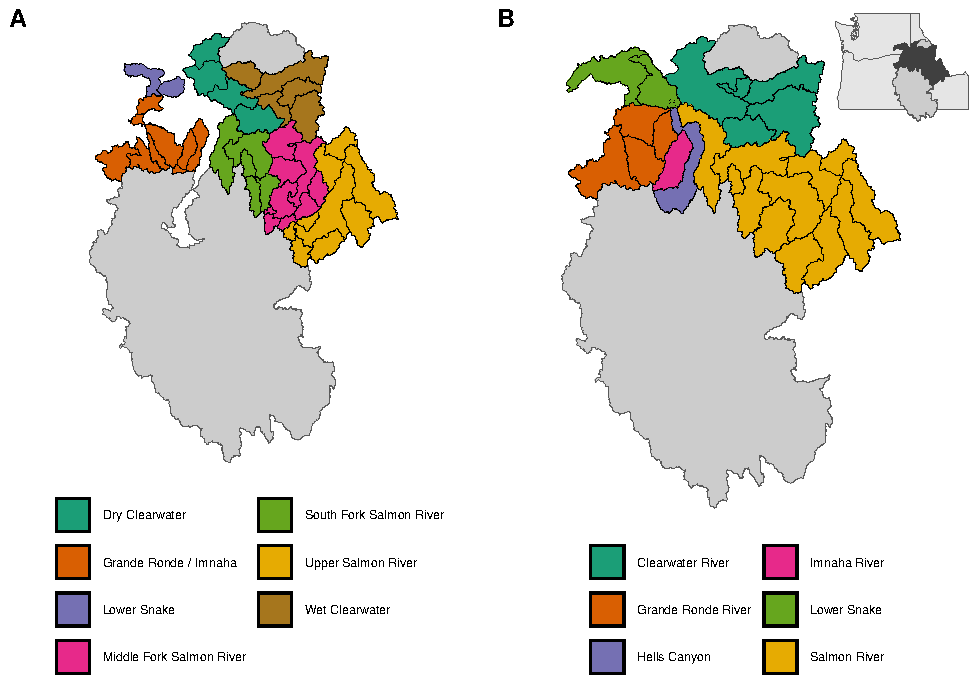
\includegraphics{manuscript_SRAFS_files/figure-latex/esu-map-1.pdf}
\caption{\label{fig:esu-map}Currently accessible and extant spring-summer Chinook Salmon (A) and steelhead (B) populations within the Snake River Basin evolutionary significant unit (ESU) or distinct population segment (DPS) are grouped in similar colors while the grey shape indicates extict populations.}
\end{figure}

\section{Methods}\label{methods}

\subsection{Data}\label{data}

This study seeks to use the best available abundance estimates of natural-origin fish returning to accessible populations within the Snake River Basin. We begin with two independent time-series of abundance estimates generated from different data collection methods and analyses completed by biologists at the Idaho Department of Fish Game, Washington Department of Fish and Game, Oregon Department of Fish and Game, and Nez Perce Tribe. We obtained both time-series from \href{https://cax.streamnet.org}{StreamNet's Coordinated Assessments} natural-origin spawner abundance (NOSA) dataset (Tables \ref{tab:chn-obs} and \ref{tab:sth-obs}). Both datasets were first subset the to include only records from Snake River Basin ESU/DPS populations, and to begin in 1980 for sp/su Chinook Salmon and 2010 for steelhead. The time period for sp/su Chinook Salmon was selected in order to only include returns years post Lower Granite Dam construction to better represent contemporary returns. The steelhead dataset begins later and aligns with the majority of steelhead data collection efforts across the Snake Basin.

The first time-series of abundance estimates were primarily derived from observations of redds and fish sampled at weirs, and intended to represent NOSA including age-3 jacks (NOSAij). In general, redd data was expanded into spawner abundance values using sex ratios estimated from carcasses and assumed fish-per-redd values (e.g., \textbf{need citation\ldots Hassemer??}), or mark-recapture studies using fish collected at weirs (e.g., \textbf{need citations}).Specifc details regarding the estimation of NOSAij for each population can be found in agency reports {[}\textbf{need citations}{]} or by contacting the contributing source listed in Coordinated Assessments metadata.

The second time-series represents escapement of natural-origin fish (including age-3 jacks) returning to the population. Population escapement estimates were derived from the STate-space Adult Dam Escapement Model (STADEM) \autocite{see_state-space_2021} and the Dam Adult Branch Occupancy Model (DABOM) \autocite{waterhouse_bayesian_2020,see_pit_2016,kinzer_snake_2020}. STADEM estimates natural and hatchery origin escapement of fish passing Lower Granite Dam. DABOM estimates time-varying transition probabilities to Snake River populations with randomly marked fish trapped at Lower Granite Dam while accounting for 1) differential adult run timings among populations and 2) potentially inconsistent trapping and tagging rates. The product of the two models equal population escapement estimates.

\begin{table}
\centering
\caption{\label{tab:chn-obs}Summary of abundance time-series used in modeling Snake River spring/summer Chinook Salmon populations (n = 48). Time-series length and data sources varied by population, with observations spanning from 1980 to 2024. Abundance estimates were primarily based on spawning ground surveys and weir counts, with PIT-tag detections included for select populations. The 10th, 50th (median), and 90th percentiles of observed abundance values are provided to summarize distributional characteristics across years.}
\centering
\fontsize{8}{10}\selectfont
\begin{tabular}[t]{llllrrrr}
\toprule
MPG & Population & Method & Years & \# Years & 10\% & 50\% & 90\%\\
\midrule
Dry Clearwater & Upper South Fork Clearwater & PIT-tag & 2012-2024 & 12 & 144 & 273 & 757\\

 & Big Sheep Creek & PIT-tag & 2011-2024 & 13 & 20 & 49 & 120\\

 &  & SGS and Weir & 1980-2024 & 45 & 36 & 129 & 527\\

 & \multirow[t]{-2}{*}{\raggedright\arraybackslash Catherine Creek} & PIT-tag & 2015-2024 & 9 & 90 & 132 & 361\\

 &  & SGS and Weir & 1980-2024 & 45 & 14 & 56 & 187\\

 & \multirow[t]{-2}{*}{\raggedright\arraybackslash Grande Ronde River Upper Mainstem} & PIT-tag & 2018-2024 & 6 & 16 & 33 & 71\\

 &  & SGS and Weir & 1980-2024 & 45 & 189 & 417 & 1028\\

 & \multirow[t]{-2}{*}{\raggedright\arraybackslash Imnaha River Mainstem} & PIT-tag & 2011-2024 & 13 & 222 & 483 & 1062\\

 & Lookingglass Creek & PIT-tag & 2010-2024 & 14 & 38 & 88 & 228\\

 & Minam River & SGS and Weir & 1980-2024 & 45 & 141 & 327 & 684\\

 & Wallowa/Lostine Rivers & SGS and Weir & 1980-2023 & 44 & 72 & 300 & 1018\\

 &  & SGS and Weir & 1980-2024 & 45 & 61 & 279 & 652\\

\multirow[t]{-12}{*}[7\dimexpr\aboverulesep+\belowrulesep+\cmidrulewidth]{\raggedright\arraybackslash Grande Ronde / Imnaha} & \multirow[t]{-2}{*}{\raggedright\arraybackslash Wenaha River} & PIT-tag & 2019-2024 & 5 & 119 & 133 & 404\\

 &  & SGS and Weir & 1984-2016 & 33 & 0 & 4 & 18\\

 & \multirow[t]{-2}{*}{\raggedright\arraybackslash Asotin Creek} & PIT-tag & 2010-2024 & 14 & 0 & 19 & 123\\

\multirow[t]{-3}{*}[1\dimexpr\aboverulesep+\belowrulesep+\cmidrulewidth]{\raggedright\arraybackslash Lower Snake} & Tucannon River & SGS and Weir & 1980-2024 & 45 & 26 & 213 & 611\\

 &  & SGS and Weir & 1980-2024 & 45 & 85 & 244 & 880\\

 & \multirow[t]{-2}{*}{\raggedright\arraybackslash Bear Valley Creek} & PIT-tag & 2015-2024 & 9 & 10 & 232 & 648\\

 &  & SGS and Weir & 1980-2024 & 45 & 38 & 131 & 417\\

 & \multirow[t]{-2}{*}{\raggedright\arraybackslash Big Creek} & PIT-tag & 2012-2024 & 12 & 198 & 585 & 1121\\

 & Camas Creek & SGS and Weir & 1980-2024 & 44 & 9 & 43 & 104\\

 & Chamberlain Creek & SGS and Weir & 1985-2024 & 36 & 30 & 187 & 526\\

 & Loon Creek & SGS and Weir & 1980-2024 & 44 & 10 & 53 & 107\\

 & Marsh Creek & SGS and Weir & 1980-2024 & 45 & 31 & 167 & 578\\

 & Middle Fork Salmon River Lower Mainstem & SGS and Weir & 1987-2024 & 37 & 0 & 3 & 23\\

 & Middle Fork Salmon River Upper Mainstem & SGS and Weir & 1995-2024 & 30 & 21 & 57 & 154\\

\multirow[t]{-11}{*}[8\dimexpr\aboverulesep+\belowrulesep+\cmidrulewidth]{\raggedright\arraybackslash Middle Fork Salmon River} & Sulphur Creek & SGS and Weir & 1980-2024 & 45 & 6 & 41 & 182\\

 &  & SGS and Weir & 1987-2024 & 38 & 62 & 212 & 503\\

 & \multirow[t]{-2}{*}{\raggedright\arraybackslash East Fork South Fork Salmon River} & PIT-tag & 2010-2024 & 14 & 243 & 629 & 1079\\

 &  & SGS and Weir & 1996-2024 & 29 & 161 & 434 & 1045\\

 & \multirow[t]{-2}{*}{\raggedright\arraybackslash Secesh River} & PIT-tag & 2010-2024 & 14 & 270 & 666 & 1191\\

 &  & SGS and Weir & 1980-2024 & 45 & 162 & 551 & 1235\\

\multirow[t]{-6}{*}[2\dimexpr\aboverulesep+\belowrulesep+\cmidrulewidth]{\raggedright\arraybackslash South Fork Salmon River} & \multirow[t]{-2}{*}{\raggedright\arraybackslash South Fork Salmon River} & PIT-tag & 2010-2024 & 14 & 213 & 675 & 2534\\

 & East Fork Salmon River & SGS and Weir & 1980-2024 & 45 & 18 & 219 & 630\\

 &  & SGS and Weir & 1980-2024 & 45 & 60 & 142 & 363\\

 & \multirow[t]{-2}{*}{\raggedright\arraybackslash Lemhi River} & PIT-tag & 2010-2024 & 14 & 129 & 235 & 665\\

 &  & SGS and Weir & 1991-2024 & 34 & 6 & 52 & 184\\

 & \multirow[t]{-2}{*}{\raggedright\arraybackslash North Fork Salmon River} & PIT-tag & 2016-2024 & 7 & 40 & 60 & 211\\

 & Pahsimeroi River & SGS and Weir & 1980-2024 & 37 & 24 & 122 & 354\\

 & Panther Creek & PIT-tag & 2018-2024 & 6 & 93 & 166 & 303\\

 & Salmon River Lower Mainstem & SGS and Weir & 1980-2024 & 45 & 19 & 98 & 230\\

 & Salmon River Upper Mainstem & SGS and Weir & 1980-2024 & 45 & 100 & 326 & 679\\

 &  & SGS and Weir & 1980-2024 & 45 & 13 & 77 & 229\\

 & \multirow[t]{-2}{*}{\raggedright\arraybackslash Valley Creek} & PIT-tag & 2010-2024 & 14 & 87 & 242 & 484\\

 &  & SGS and Weir & 1980-2024 & 44 & 3 & 23 & 148\\

\multirow[t]{-13}{*}[8\dimexpr\aboverulesep+\belowrulesep+\cmidrulewidth]{\raggedright\arraybackslash Upper Salmon River} & \multirow[t]{-2}{*}{\raggedright\arraybackslash Yankee Fork} & PIT-tag & 2012-2024 & 12 & 35 & 62 & 279\\

 & Lochsa River & PIT-tag & 2017-2024 & 7 & 160 & 245 & 461\\

\multirow[t]{-2}{*}[1\dimexpr\aboverulesep+\belowrulesep+\cmidrulewidth]{\raggedright\arraybackslash Wet Clearwater} & Lolo Creek & PIT-tag & 2012-2024 & 12 & 41 & 78 & 257\\
\bottomrule
\end{tabular}
\end{table}

\begin{table}
\centering
\caption{\label{tab:sth-obs}Summary of abundance time-series used in modeling Snake River summer steelhead populations (n = 25). Time-series length and data sources varied by population, with observations spanning from 2010 to 2024. Abundance estimates were primarily based on PIT-tag detections, with spawning ground surveys and weir counts included for select populations. The 10th, 50th (median), and 90th percentiles of observed abundance values are provided to summarize distributional characteristics across years.}
\centering
\fontsize{8}{10}\selectfont
\begin{tabular}[t]{llllrrrr}
\toprule
MPG & Population & Method & Years & \# Years & 10\% & 50\% & 90\%\\
\midrule
 & Clearwater River Lower Mainstem & SGS and Weir & 2010-2024 & 15 & 147 & 254 & 785\\

 & Lochsa River & SGS and Weir & 2017-2024 & 8 & 289 & 439 & 941\\

 & Lolo Creek & SGS and Weir & 2012-2024 & 13 & 104 & 187 & 589\\

 & Selway River & SGS and Weir & 2017-2024 & 8 & 232 & 408 & 802\\

\multirow[t]{-5}{*}[4\dimexpr\aboverulesep+\belowrulesep+\cmidrulewidth]{\raggedright\arraybackslash Clearwater River} & South Fork Clearwater River & SGS and Weir & 2012-2024 & 13 & 131 & 353 & 1040\\

 & Grande Ronde River Lower Mainstem & SGS and Weir & 2019-2023 & 5 & 281 & 418 & 467\\

 &  & SGS and Weir & 2013-2024 & 12 & 356 & 539 & 1301\\

 & \multirow[t]{-2}{*}{\raggedright\arraybackslash Grande Ronde River Upper Mainstem} & PIT-tag & 2010-2018 & 9 & 1300 & 2556 & 3589\\

 &  & SGS and Weir & 2011-2024 & 14 & 372 & 747 & 2045\\

 & \multirow[t]{-2}{*}{\raggedright\arraybackslash Joseph Creek} & PIT-tag & 2010-2017 & 8 & 1487 & 1990 & 3735\\

\multirow[t]{-6}{*}[3\dimexpr\aboverulesep+\belowrulesep+\cmidrulewidth]{\raggedright\arraybackslash Grande Ronde River} & Wallowa River & SGS and Weir & 2014-2024 & 11 & 359 & 508 & 956\\

Imnaha River & Imnaha River & SGS and Weir & 2011-2024 & 14 & 683 & 1241 & 2881\\

 & Asotin Creek & SGS and Weir & 2010-2024 & 15 & 224 & 366 & 1312\\

 &  & SGS and Weir & 2010-2024 & 15 & 232 & 452 & 841\\

\multirow[t]{-3}{*}[1\dimexpr\aboverulesep+\belowrulesep+\cmidrulewidth]{\raggedright\arraybackslash Lower Snake} & \multirow[t]{-2}{*}{\raggedright\arraybackslash Tucannon River} & PIT-tag & 2010-2023 & 14 & 347 & 611 & 1196\\

 & East Fork Salmon River & SGS and Weir & 2011-2019 & 8 & 0 & 14 & 40\\

 & Lemhi River & SGS and Weir & 2010-2024 & 15 & 49 & 161 & 416\\

 & Middle Fork Salmon River Lower Mainstem & SGS and Weir & 2011-2024 & 14 & 84 & 244 & 586\\

 & Middle Fork Salmon River Upper Mainstem & SGS and Weir & 2020-2024 & 5 & 19 & 29 & 53\\

 & North Fork Salmon River & SGS and Weir & 2017-2024 & 7 & 17 & 57 & 378\\

 & Pahsimeroi River & SGS and Weir & 2011-2024 & 14 & 9 & 33 & 140\\

 & Panther Creek & SGS and Weir & 2018-2024 & 7 & 101 & 137 & 196\\

 & Salmon River Upper Mainstem & SGS and Weir & 2010-2024 & 15 & 36 & 106 & 297\\

 & Secesh River & SGS and Weir & 2010-2024 & 15 & 27 & 57 & 252\\

\multirow[t]{-10}{*}[9\dimexpr\aboverulesep+\belowrulesep+\cmidrulewidth]{\raggedright\arraybackslash Salmon River} & South Fork Salmon River & SGS and Weir & 2010-2024 & 15 & 154 & 445 & 1511\\
\bottomrule
\end{tabular}
\end{table}

{[}Figure of stochasiticity across time, and the synchronization after 1980.{]}

\subsection{Abundance Patterns}\label{abundance-patterns}

In each case, the time-series abundance data are not the exact truth, and in many cases, they are reported without levels of certainty (i.e., precision estimates) or measurement error. Reported estimates instead are generally the result of incomplete observations (i.e., spatial and temporal coverage is incomplete) and the product of combining information from multiple data collection activities and fish metrics together (i.e., redd count surveys, mark/recapture events, carcass collections), with each item having the possibility of being incorrect or biasing the abundance estimate from the unknown truth \autocite{auger-methe_guide_2021}. To better understand the true unknown abundance and underlying trends contained within the data we removed measurement error using a multivariate dynamic linear model (DLM) \autocite{zuur_estimating_2003}. A DLM is a time series model constructed as a type of state-space model that separates observation and state processes, and assumes the processes change dynamically following linear models \autocite{royle_hierarchical_2008}. Dynamic linear models are capable of capturing the serial correlation in the data and can share covariance across multiple time-series, thus, effectively allowing information to be shared from data rich populations with long time-series, to data poor populations with short datasets or missing years \autocite{auger-methe_guide_2021,holmes_marss_2012}. Although DLMs can handle some missing data, we conservatively chose to only include time-series with five or more years of abundances to reduce potential risks of parameter bias and overfitting.

The unobserved state process model follows the linear equation,

\[
x_t = x_{t-1} + u + w_t; \\
w_t \sim MVN(0,\mathbf{Q})
\]
where, \(x_t\) is an \(m \space X \space 1\) matrix of true unknown states for return year \(t\). Parameter \(u\) is \(m \space X \space 1\) and represents drift between subsequent return years for each state \(m\). Process error (\(w_t\)) is assumed multivariate normal with mean zero and the \(m \space X \space m\) variance-covariance matrix \(\bf{Q}\).

The observation model is represented as,

\[
y_t = \mathbf{Z}x_t + a + v_t; \\
v_t \sim MVN(0,\mathbf{R})
\]
where, \(y_t\) is an \(n \space X \space 1\) matrix of natural-log transformed observed abundance at return year \(t\) for \(n\) independent time-series. Return year abundances for each \(n\) and \(t\) observation is mapped to the unknown state (\(x_t\)) with the \(n \space X \space m\) matrix \(\bf{Z}\). Parameter \(a\) is \(n \space X \space 1\) and provides a y-intercept scaling (i.e., bias correction) for the \(m^{th}\) state and each \(n^{th}\) time-series. Observational error (\(v_t\)) is modeled as multivariate normal with mean zero and the \(n \space X \space n\) variance-covariance matrix \(\bf{R}\).

We modeled four different scenarios to represent true unknown states for sp/su Chinook Salmon and steelhead populations. The scenarios included an individual state for each of the \(n\) time-series, states for each of the populations, states for each of the major population groups (MPGs), and a single state for the entire Snake River Basin. Parameters \(u\) and \(a\) were set to unequal across the modeled states and time-series mapped to each state.

We modeled three different variance-covariance matrices for process error and two variance-covariance matrices of observation error for each of the four state scenarios. The process error matrix (\(\bf{Q}\)) was assumed to eithr have equal variance and covariance terms for each state, or no covariance and equal or unequal variances on the matrix diagonal. The observation error matrix (\(\bf{R}\)) was assumed to have either equal or unequal variance on the diagonal, while off diagonal covariance terms were equal to zero.

The different combinations resulted in 14 model runs fit with the MARSS package \autocite{holmes_marss_2012} and the statistical programming language R \autocite{R-base}. The best model was selected as having the lowest AICc value of all successful (i.e., converged) model runs \autocite{holmes_marss_2012,R-MARSS}. Residuals from selected models were examined visually for assumption violations of heterogeneity and normality. All models were fit using the statistical software R \autocite{R-base} and the MARSS package \autocite{holmes_marss_2012,R-MARSS}.

\subsection{Recent 10-year Trends}\label{recent-10-year-trends}

To evaluate recent population trajectories, we calculated a 10-year trend for each population, representing the most recent two generations of returns. Limiting the analysis to the past decade allowed us to focus on population responses to recent environmental conditions while retaining sufficient interannual variability in abundance.

For each population, the trend was estimated from the state process (\(x_t\)), produced by the best fitting DLM, to which the population was assigned. The trend was calculated as the slope of a linear regression of the estimated natural-log-transformed abundance (\(x_t\)) on year. The slope represents the average annual rate of change in abundance over the past 10 years.

\subsection{Population Status}\label{population-status}

We assessed current and projected population status by evaluating the proportion of populations above or below abundance evaluation points (e.g., ``healthy and harvestable'', minimum viable threshold, or QET). A population was considered below the QET if its estimated abundance from the DLM fell below 50 in each of the last four years of observation (2021-2024). The proportion was calculated as the number of populations within each abundance criterion divided by the total number of populations included in the DLM analysis.

Future population status was assessed using 5-year forecasts using the slope parameter from the linear regression models described above. A population was classified as falling below the QET if any single year within the forecast period was predicted to be below 50 spawners, under the assumption that all subsequent values would remain below the threshold due to the linear nature of the model.

\section{Results}\label{results}

\subsection{Abundance Patterns}\label{abundance-patterns-1}

The best fitting model for sp/su Chinook Salmon included separate state processes for each major population group (Table \ref{tab:chn-mod-results}), whereas, summer steelhead was best represented by a single basin-wide process (Table \ref{tab:sth-mod-results}). For both species, the difference in AICc values between the top two models exceeded 10.00, a threshold commonly interpreted to indicate the second ranked model has little to no support as compared to the first ranked model \autocite{burnham_multimodel_2004}. For sp/su Chinook Salmon, the process error matrix included two parameters: one for an equal variance and the other for an equal covariance across the seven MPG processes. In contrast, the best fitting model for summer steelhead included only a single basin-wide process, as such, process error consisted of a single variance parameter. Observational error for both species was best modeled with unique variance parameters for each time-series.

We evaluated model assumptions by visually examining residual plots for patterns indicating autocorrelation, non-normality, or heteroscedasticity. Overall, these diagnostic checks supported the adequacy of the model structure and parameter estimates (Figures \ref{fig:chn-resids} and \ref{fig:sth-resids}). However, in a few populations residuals did show evidence of serial correlation and any future models may benefit from additional terms. Model convergence was confirmed with the MARSS package output indicating the optimization algorithm reached a stable peak in the likelihood \autocite{holmes_2021}.

\begin{table}

\caption{Candidate dynamic linear models fitted to 48 spring/summer Chinook Salmon abundance time-series to evaluate population dynamics and identify models best explaining Snake River trends. The number of state processes estimated in each model is indicated in column U. Unique state process error parameters are denoted in column Q, and observation error parameters in column R. Model fit is summarized using log-likelihood (logLik), corrected Akaike Information Criterion (AICc), and relative model support ($\Delta$AIC).}
\centering
\begin{tabular}[t]{rrrrrrr}
\toprule
Model Id & U & Q & R & logLik & AICc & $\Delta$AIC\\
\midrule
4 & 7 & 2 & 48 & -1409.39 & 3048.45 & 0.00\\
2 & 1 & 1 & 48 & -1466.43 & 3146.20 & 97.75\\
10 & 34 & 2 & 48 & -1434.48 & 3163.32 & 114.87\\
8 & 7 & 7 & 48 & -1483.20 & 3207.85 & 159.39\\
6 & 7 & 1 & 48 & -1497.10 & 3221.52 & 173.07\\
\addlinespace
3 & 7 & 2 & 1 & -1592.07 & 3307.45 & 259.00\\
1 & 1 & 1 & 1 & -1644.39 & 3396.90 & 348.45\\
9 & 34 & 2 & 1 & -1619.06 & 3421.60 & 373.15\\
7 & 7 & 7 & 1 & -1658.74 & 3451.76 & 403.30\\
5 & 7 & 1 & 1 & -1675.38 & 3471.89 & 423.44\\
\addlinespace
14 & 34 & 34 & 48 & -1652.97 & 3680.66 & 632.20\\
12 & 34 & 1 & 48 & -1710.60 & 3713.10 & 664.65\\
13 & 34 & 34 & 1 & -1787.79 & 3833.66 & 785.20\\
11 & 34 & 1 & 1 & -1894.17 & 3969.55 & 921.09\\
\bottomrule
\end{tabular}
\end{table}

\begin{table}

\caption{Candidate dynamic linear models fitted to 25 summer steelhead abundance time-series to evaluate population dynamics and identify models best explaining Snake River trends. The number of state processes estimated in each model is indicated in column U. Unique state process error parameters are denoted in column Q, and observation error parameters in column R. Model fit is summarized using log-likelihood (logLik), corrected Akaike Information Criterion (AICc), and relative model support ($\Delta$AIC).}
\centering
\begin{tabular}[t]{rrrrrrr}
\toprule
Model Id & u & Q & R & logLik & AICc & $\Delta$AIC\\
\midrule
2 & 1 & 1 & 25 & -173.6063 & 477.5700 & 0.00000\\
4 & 5 & 2 & 25 & -172.4959 & 490.7482 & 13.17829\\
10 & 22 & 2 & 25 & -152.4930 & 508.5072 & 30.93727\\
6 & 5 & 1 & 25 & -197.1921 & 537.0077 & 59.43771\\
8 & 5 & 5 & 25 & -195.7174 & 546.7564 & 69.18648\\
\addlinespace
1 & 1 & 1 & 1 & -290.3841 & 645.4864 & 167.91640\\
12 & 22 & 1 & 25 & -227.4331 & 654.7353 & 177.16530\\
3 & 5 & 2 & 1 & -290.2449 & 657.8599 & 180.28994\\
9 & 22 & 2 & 1 & -279.5091 & 683.3980 & 205.82803\\
7 & 5 & 5 & 1 & -304.4895 & 694.1822 & 216.61226\\
\addlinespace
5 & 5 & 1 & 1 & -313.8774 & 702.5548 & 224.98481\\
13 & 22 & 22 & 1 & -258.2618 & 705.6388 & 228.06887\\
11 & 22 & 1 & 1 & -300.5271 & 722.4827 & 244.91276\\
14 & 22 & 22 & 25 & -221.9866 & 728.4811 & 250.91111\\
\bottomrule
\end{tabular}
\end{table}

The estimated annual percent change in abundance over the full time series (\(u\)), calculated as \((e^u - 1) \times 100\), ranged from -9.52\% and 2.84\% for spring-summer Chinook Salmon (1980-2024) and summer steelhead (2010-2024; Figures \ref{fig:chn-state} and \ref{fig:sth-state}). Among the Chinook Salmon populations, those within the Lower Snake major population group (i.e., Asotin Creek and Tucannon River) exhibited the fastest rate of decline, with an estimated annual decrease of -5.8\%. In contrast, the highest positive growth was observed in populations from the South Fork Salmon River major population group. Summer steelhead had the steepest overall decline, with an estimated annual growth rate of -9.52\%.

\begin{figure}
\includegraphics[width=1\linewidth]{../figures/Chinook_salmon/Chinook_salmon_states_2024} \caption{Estimated abundance (natural-log) trends for the seven state processes (xtT) estimated from the best fitting Snake River spring/summer Chinook Salmon model (grey shading represents 95\% CI's). The abundance trend for each process across the full time-series is shown by the dashed line and generated from the estimated u and x0 parameters.}\label{fig:chn-state}
\end{figure}

\begin{figure}
\includegraphics[width=1\linewidth]{../figures/Steelhead/Steelhead_states_2024} \caption{Estimated abundance (natural-log) trend for a single state process (xtT) as estimated from the best fitting Snake River summer steelhed model (grey shading represents 95\% CI's). The abundance trend for each process across the full time-series is shown by the dashed line and generated from the estimated u and x0 parameters.}\label{fig:sth-state}
\end{figure}

\subsection{Recent 10-year Trends}\label{recent-10-year-trends-1}

After fitting a linear regression line to the last 10-years of estimated state processes we found summer steelhead has decreased annually by 11\% and six spring-summer Chinook Salmon major population groups also decreased (Figures \ref{fig:chn-sa-slope} and \ref{fig:sth-sa-slope}). Again, the Chinook Salmon South Fork Salmon River major population group had the highest, and only positive, rate of growth at 5.13\% annually. The remaining six major population groups in the last 10 years have decreased at annual rates of 5\% and higher, with the most severe decrease being 13\% in the Lower Snake populations.

\begin{figure}
\includegraphics[width=1\linewidth]{../figures/Chinook_salmon/Chinook_salmon_slope_2024} \caption{Estimated slope parameters for natural-origin Snake River spring/summer Chinook Salmon abundance trends indicate an average annual decline of 6\% for the last 10-years.}\label{fig:chn-sa-slope}
\end{figure}

\begin{figure}
\includegraphics[width=1\linewidth]{../figures/Steelhead/Steelhead_slope_2024} \caption{Modeled abundance trends of natural-origin Snake River summer steelhead indicate an annual 11\% decline for the last 10-years.}\label{fig:sth-sa-slope}
\end{figure}

\subsection{Population Status}\label{population-status-1}

Over the last 45 return years included in the sp/su Chinook Salmon analysis most abundances have been below critical levels. Of the 1530 combinations of populations and return years, 0 of the returns have been at ``healthy and harvestable levels'', and only 122 (8\%) have been above minimum abundance thresholds, while 323 (21\%) have been below 50 annual spawners (Figure \ref{fig:chn-targets}).

The mean return of the last four years of sp/su Chinook Salmon population abundances only account for an average of 23\% of MAT across all populations. Four populations of sp/su Chinook Salmon currently meet the requirements of quasi-extinction (i.e., four consecutive years below 50 spawners) and an additional 8 populations were below 50 in 2024. While another 2 are predicted to drop below 50 by 2029, ultimately resulting in 41\% of the analyzed sp/su Chinook Salmon populations being predicted to reach quasi-extinction within the next 5 years (Figure \ref{fig:chn-qet-map}).

\begin{figure}
\includegraphics[width=1\linewidth]{../figures/Chinook_salmon/Chinook_salmon_map_2024} \caption{Current status of natural-origin Snake River spring/summer Chinook Salmon relative to the quasi-extinction threshold (QET) and Columbia Basin Partnership goals.}\label{fig:chn-qet-map}
\end{figure}

Across the last 15 return years included in the analysis, steelhead abundances have also remained low relative to goals. Out of 330 total population-year combinations, 4 were at ``healthy and harvestable'' levels, 81 exceeded the minimum abundance thresholds, and 43 (13\%) of all records were at critical abundance levels (Figure \ref{fig:sth-targets}).

The average steelhead abundance over the most recent four year period has a mean return representing just 36\% of the minimum abundance threshold across all populations. Currently, three steelhead populations meet the QET criteria, and an additional three populations are projected to fall below this threshold by 2029. In total, 27\% of the analyzed steelhead populations are expected to reach quasi-extinction within the next five years (Figure \ref{fig:sth-qet-map}).

\begin{figure}
\includegraphics[width=1\linewidth]{../figures/Steelhead/Steelhead_map_2024} \caption{Current status of natural-origin Snake River summer steelhead relative to the quasi-extinction threshold (QET) and Columbia Basin Partnership goals.}\label{fig:sth-qet-map}
\end{figure}

\section{Discussion}\label{discussion}

Despite over three decades of recovery actions since the ESA listing of Snake River sp/su Chinook Salmon and steelhead, our results show that most extant populations remain well below viable abundance thresholds and far from healthy or harvestable levels. Notably, seven populations---four Chinook and three steelhead---currently meet the quasi-extinction threshold (QET) of 50 or fewer spawners for the past four consecutive years. If current 10-year trends persist, an additional 13 populations are projected to fall below the QET within five years. These findings are particularly concerning given the magnitude of recovery investments, including hydrosystem passage improvements, large-scale habitat restoration, and hatchery supplementation programs. In contrast to the intended outcomes, Snake River populations appear to have lost ground in the fight against extinction.

Over the last 10 years, sp/su Chinook Salmon and steelhead abundances have declined more sharply than in prior decades. Abundance estimates suggests that the most recent downward trend in both species began in 2010. These patterns are consistent with research showing strong correlations between salmon returns and oceanographic conditions such as the Pacific Decadal Oscillation and sea surface temperatures \autocite{mantua_pacific_1997,crozier_climate_2021}. As ocean conditions continue to warm, further declines are likely without substantial changes to freshwater conditions.

While both species have shown some variability in annual returns, long-term averages remain below recovery targets. Since ESA listing, sp/su Chinook Salmon populations have exceeded the minimum abundance threshold only in 8\% of the return years, and recent returns have hovered near QET levels. Steelhead populations have exceeded MAT more frequently but remain far from delisting thresholds or Columbia Basin Partnership goals for healthy and harvestable populations.

We replicated and slightly modified \textcite{ford_biological_2022} modeling framework to estimate underlying population dynamics to assess and update Snake River anadromous population trends. We chose a 10-year evaluation window, starting in 2015, to capture the more recent and steeper declines visible in both sp/su Chinook Salmon and steelhead abundance. Unlike \textcite{ford_biological_2022} 15-year trend approach, which we believe may have masked current declines due to low starting and ending points (i.e., a less steep slope), our analysis focused on the more immediate trajectory of population change, providing a more sobering and urgent picture of current status.

Indeed, we found nearly all sp/su Chinook Salmon populations had declined from 2015-2024---a 6\% average annual decrease. Steelhead populations declined slightly faster at an annual rate 18\%. Four (12\%) of the sp/su Chinook Salmon populations are already below the quasi-extinction threshold, and 14 (41\%) are projected to be quasi-extinct within five years. Fewer steelhead populations (3, or 14\%) are currently at the quasi-extinct level, but projections indicate that 6 (27\%) will reach this threshold within five years.

These results suggest that Snake River anadromous fish populations are responding similarly to broad-scale environmental drivers rather than localized habitat conditions. This aligns with previous findings that populations within major population groups are often exposed to similar migration barriers, ocean conditions, and management actions \autocite{copeland_how_2024}. The fitted models showed population time series have mostly decreased since the beginning of the datasets, with recent declines driving projected quasi-extinction risk. Notably, the Lower Snake and Wet Clearwater major population groups for sp/su Chinook Salmon---areas of lower elevation and more degraded habitat---showed the fastest rates of decline.

The predictive models used here assume the recent 10-year trend continues linearly. While this simplification ignores serial correlation and potential reversals due to cyclic conditions (e.g., improved ocean years), it effectively highlights the long-term trajectory under a ``status quo'' scenario. For instance, the higher-than-expected returns observed in 2021 and 2022 likely reflect short-term improvements in ocean conditions and do not alter the long-term trend of decline. Importantly, even these higher returns remain well below the thresholds necessary for delisting or for reaching recovery goals.

\subsection{Conclusions and Implications}\label{conclusions-and-implications}

Since ESA listing, billions of dollars have been invested in recovery, yet Snake River Chinook and steelhead populations have failed to rebound. While localized benefits from habitat projects and passage improvements have been observed, they have not altered basinwide trends. Our analysis confirms that most populations are either below or approaching extinction thresholds, and the underlying causes---particularly ocean survival and hydrosystem-related mortality---remain largely unaddressed.

Looking ahead, climate change poses an even greater challenge. Warmer ocean conditions and reduced snowpack are expected to reduce freshwater flows, increase stream temperatures, and exacerbate mortality throughout the fishes' life cycle \autocite{crozier_climate_2019,crozier_climate_2021}. Given these pressures, even more aggressive actions may be necessary to avoid extinction. This includes both structural changes (e.g., breaching Lower Snake River dams to improve passage and habitat) and conservation interventions (e.g., temporary supplementation, captive broodstocks, or revised harvest policies) to prevent the loss of populations before long-term solutions can take effect.

In summary, our analysis provides a scientifically grounded, transparent evaluation of the current and projected status of Snake River anadromous fish. While short-term variability will persist, the long-term trend is unmistakable: these populations are declining. Without bold and transformative action, ESA recovery goals will remain out of reach, and the region may lose the opportunity to sustain wild salmon and steelhead for future generations.

\section{Code and Data Availability}\label{code-and-data-availability}

The code and processed data to reproduce the analyses, summaries, tables, and figures are available on the GitHub project repository at \url{https://github.com/ryankinzer/SRAFS.git}. Raw time-series observation data are available from Stream Net's Coordinated Assessments Indicators of Fish Population Health web application; \url{https://cax.streamnet.org}.

\section{Acknowledgements}\label{acknowledgements}

Providing the current status of Snake River fish stocks would not be possible without the gigantic efforts of hundreds of biologists, technicians, and field crews who have collected monitoring data across the basin over the past three decades. We are especially grateful to the many tribal, state, and federal agency staff whose long-term dedication to data collection, stewardship, and recovery efforts have provided the foundation for this analysis. We also thank the regional biologists and data managers who ensured the consistency and integrity of datasets spanning multiple generations of monitoring programs. Evan Brown, Rebecca Waskovich and Luciano Chiramonte from Idaho Department of Fish and Game, Joseph Feldhaus and Kasey Bliesner from Oregon Department of Fish and Wildlife, and Ethan Crawford and Michael Gallinat from Washington Department of Fish and Wildlife deserve a special thanks for meeting our data requests and helping us understand the methods and nuances. We thank our, now retired, program manager, David B. Johnson, for encouraging this work and using it to guide future recovery decisions and inform policy makers. Manuscript review and guidance pre-journal submittal were generously provided by \textbf{placeholder}, \textbf{placeholder}, \textbf{placeholder}, and \textbf{placeholder}. We also extend our gratitude to the anonymous journal reviewers whose thoughtful feedback greatly improved the quality and clarity of this manuscript.

\clearpage

\section{References}\label{references}

\printbibliography[heading=none]
\def\printbibliography{}

\clearpage

\appendix
\renewcommand{\thefigure}{S\arabic{figure}}  % Number figures as S1, S2, ...
\setcounter{figure}{0}

\section{Supplemental Material}\label{supplemental-material}

\begin{figure}[H]
\includegraphics[width=1\linewidth]{../figures/Chinook_salmon/Chinook_salmon_residuals_2024} \caption{Residuals from the best fitting spring-summer Chinook Salmon MARSS model.}\label{fig:chn-resids}
\end{figure}

\begin{figure}[H]
\includegraphics[width=1\linewidth]{../figures/Steelhead/Steelhead_residuals_2024} \caption{Residuals from the best fitting summer steelhead MARSS model.}\label{fig:sth-resids}
\end{figure}

\begin{figure}
\includegraphics[width=1\linewidth]{../figures/Chinook_salmon/Chinook_salmon_pop_thresholds_2024} \caption{Modeled abundance estimates of natural-origin Snake River spring/summer Chinook Salmon relative to the quasi-extinction, minimum viable abundance, and health and harvestable thresholds.}\label{fig:chn-targets}
\end{figure}

\begin{figure}
\includegraphics[width=1\linewidth]{../figures/Steelhead/Steelhead_pop_thresholds_2024} \caption{Modeled abundance estimates of natural-origin Snake River summer steelhead relative to the quasi-extinction, minimum viable abundance, and health and harvestable thresholds.}\label{fig:sth-targets}
\end{figure}

% Bibliography
\printbibliography


\end{document}
